\begin{frame}{Depth-$3$ lower bounds. $k$-limit}


    \begin{itemize}
        \item $\varphi$ is a $k$-DNF;
        \item $A \coloneqq \{a \in X \mid \varphi(a) = 1\}$;
        \item what can we say about $A$?
    \end{itemize}

    \pause

    \begin{block}{$k$-limit [H{\aa}stad, Jukna, Pudlak 95]}
        $x \in \{0, 1\}^n$ is a \deftext{$k$-limit} of $A \subseteq \{0, 1\}^n$ $\Leftrightarrow$
        $\forall I \subseteq [n]$ of size $k$, $\exists a \in A$ such that $x_I = a_I$.
    \end{block}

    \pause
    \begin{center}
        \begin{tikzpicture}
    \def\elements{{
            {1, 1, 0, 1, 1},
            {0, 1, 0, 1, 0},
            {0, 0, 1, 1, 1},
            {1, 1, 1, 1, 0},
            {1, 1, 1, 0, 1},
            {0, 1, 0, 1, 1},
            {1, 1, 1, 0, 1},
            {0, 0, 1, 0, 0},
            {1, 1, 1, 1, 1}
        }}
    \def\result{{1, 0, 1, 1, 1, 1, 1, 0, 1}} 
    \def\n{3}
    \def\m{4}
    \def\step{0.65}

    \draw[step = \step, thick] (0, 0) grid ({\step * (\n + 1)}, {-\step * (\m + 1)});
    
        
    \foreach \i in {0, 1, ..., \n}{
        \foreach \j in {0, 1, ..., \m}{
            \node at ({\step / 2 + \i * \step}, {-\step / 2 - \j * \step})
                {\pgfmathparse{\elements[\i][\j]}\pgfmathresult};
        }
    }

    \begin{scope}[shift = {(0, {-\step * (\m + 1) - 0.7})}]
        \draw[step = \step, thick] (0, 0) grid ({\step * (\n + 1)}, -\step);
        \draw[thick, green!30!black, rounded corners = 2pt,
            fill = green, fill opacity = 0.2, alt = <{4-}>{}{opacity = 0}]
            (\step - 0.02, 0 + 0.02) rectangle (4 * \step + 0.02, -\step - 0.02);
            
        \foreach \i in {0, 1, ..., \n}{
            \node at ({\step / 2 + \i * \step}, {-\step / 2})
                {\pgfmathparse{\result[\i]}\pgfmathresult};
        }
    \end{scope}

    \node at (-0.5, {-\step * (\m + 1) / 2}) {\Large $A$};
    \node at (-0.5, {-\step * (\m + 1.5) - 0.7}) {$3$-limit};

    \draw[thick, green!30!black, rounded corners = 2pt, fill = green,
        fill opacity = 0.2, alt = <{4-}>{}{opacity = 0}]
        (\step - 0.02, {-\step * 3 - 0.02}) rectangle
        ({\step * (\n + 1) + 0.02}, {-\step * 2 + 0.02});
\end{tikzpicture}
    \end{center}
\end{frame}



\begin{frame}{Spreadness}

    $X \subseteq \binom{n}{k}$ is $\delta$-spread $\Leftrightarrow
    \forall I \in [n]$:
    $$
        \Pr\limits_{x \sim \mathbf{X}}[x_I = 1_I] \le \left(\frac{k}{n}\right)^{\delta |I|}.
    $$

    \pause

    \begin{center}
        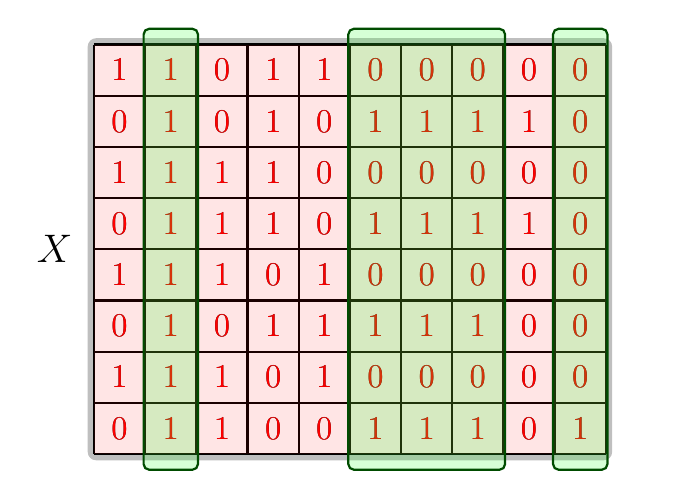
\begin{tikzpicture}
    \def\elements{{
            {1, 1, 0, 1, 1, 0, 0, 0, 0, 0},
            {0, 1, 0, 1, 0, 1, 1, 1, 1, 0},
            {1, 1, 1, 1, 0, 0, 0, 0, 0, 0},
            {0, 1, 1, 1, 0, 1, 1, 1, 1, 0},
            {1, 1, 1, 0, 1, 0, 0, 0, 0, 0},
            {0, 1, 0, 1, 1, 1, 1, 1, 0, 0},
            {1, 1, 1, 0, 1, 0, 0, 0, 0, 0},
            {0, 1, 1, 0, 0, 1, 1, 1, 0, 1}
        }}
    \def\result{{1, 0, 1, 1, 1, 1, 1, 0, 1}} 
    \def\n{9}
    \def\m{7}
    \def\step{0.65}

    \fill[gray!50, rounded corners = 3pt] (-0.08, 0.08) rectangle
        ({\step * (\n + 1) + 0.08}, {-\step * (\m + 1) - 0.08});
    \fill[white] (0, 0) rectangle ({\step * (\n + 1)}, {-\step * (\m + 1)}); 
    \draw[step = \step, thick] (0, 0) grid ({\step * (\n + 1)}, {-\step * (\m + 1)});

    \foreach \i in {0, 1, ..., \n}{
        \foreach \j in {0, 1, ..., \m}{
            \pgfmathparse{\elements[\j][\i]}
            \edef\val{\pgfmathresult}
            \ifthenelse{\val = 0}{
                \node at ({(\i + 0.5) * \step}, {-(\j + 0.5) * \step})
                    {\large \val};
            }{
                \node at ({(\i + 0.5) * \step}, {-(\j + 0.5) * \step})
                    {\textcolor{red}{\large \val}};
                \fill[red, opacity = 0.1]
                    ({\i * \step}, {-\j * \step})
                    rectangle
                    ({(\i + 1) * \step}, {-(\j + 1) * \step});
            }
        }
    }

    \uncover<2->{
        \draw[thick, green!30!black, rounded corners = 2pt, fill = green!80, fill opacity = 0.2]
            ({-0.02 + \step}, 0.2) rectangle ({\step * 2 + 0.02}, {-\step * (\m + 1) - 0.2});
    }

    \uncover<3->{
        \draw[thick, green!30!black, rounded corners = 2pt, fill = green!80, fill opacity = 0.2]
            ({-0.02 + \n * \step}, 0.2) rectangle
            ({(\n + 1) * \step + 0.02}, {-\step * (\m + 1) - 0.2});
    }

    \uncover<4->{
        \draw[thick, green!30!black, rounded corners = 2pt, fill = green!80, fill opacity = 0.2]
            ({-0.02 + 5 * \step}, 0.2) rectangle ({\step * 8 + 0.02}, {-\step * (\m + 1) - 0.2});
    }

 
    \node at (-0.5, {-\step * (\m + 1) / 2}) {\Large $X$};
    \node at ({\step * (\n + 1) + 0.5}, {-\step * (\m + 1) / 2}) {};

\end{tikzpicture}
    \end{center}

    \pause
    \pause
    \pause

    \begin{itemize}
        \item $0.9$-spread set is a robust sunflower with an empty core.
    \end{itemize}
    
\end{frame}


\begin{frame}{Spreadness $\Rightarrow$ $k$-limit}

    Let $X \subseteq \{0, 1\}^n$ collection of points of weight $k < \sqrt{n}$.
    
    \begin{lemma}    
        $X$ is $0.9$-spread $\Rightarrow$ $0$ is a $n^{0.45}$-limit.
    \end{lemma}

    \pause

    \begin{enumerate}
        \item Fix $I \subseteq [n]$ of size $k$.
        \item For each $i \in I$: $\Pr\limits_{x \sim \mathbf{X}}[x_i = 1] \le \left( k / n \right)^{0.9}
            \le n^{-0.45}$.
            \pause
        \item $\Pr\limits_{x \sim \mathbf{X}}[\exists i \in I, x_i = 1] < 1$.
    \end{enumerate}

    \pause
    \begin{corollary}
        $\Parity$ \alert{(and many other partial functions)} requires depth-$3$ circuits of size $2^{n^{\varepsilon}}$.
    \end{corollary}

    \pause
    \begin{corollary}[Santha 89]
        \alert{$\exists$} $O$ such that $\AM^{O} \nsubseteq \Sigma_2^{O}$.
    \end{corollary}

    
\end{frame}


\begin{frame}{$\Parity$ req. depth-$3$ ckt of size $2^{n^{\varepsilon}}$}

    \tikzset{
    vert/.style = {
        circle,
        thick,
        minimum size = 0.5cm
    },
    fancy-arrow/.style = {
        draw = black,
        thick,
        single arrow,
        right color = green!40!black,
        left color = red!40!black,
        fill opacity = 0.7,
        single arrow head extend = 0.3cm,
        single arrow tip angle = 70,
        single arrow head indent = 0.15cm,
        minimum height = 1.4cm,
        minimum width = 1cm,
        shading angle = -45,
        rotate = -90
    },
    common-part/.pic = {
        \draw[thick] (0, 0) rectangle (\a, \a);
        \draw[thick] (0, 0) -- (\a, \a);

        \node at (0.5, \a - 0.5) {\Large $0$};
        \node at (\a - 0.5, 0.5) {\Large $1$};

        \foreach \i in {1, 2, ..., 5}{
            \draw[thick, ->] (a) -- (b\i);
        }
    },
}
    
\begin{tikzpicture}[>=latex]
    \def\a{4}


    \fill[red!70!black, opacity = 0.3] (0, 0) -- (\a, \a) -- (\a, 0) -- cycle;
    \fill[green!50!black, opacity = 0.3] (0, 0) -- (\a, \a) -- (0, \a) -- cycle;

    \begin{scope}[shift = {(9, 0)}]
        \node[draw, vert, color = green!40!black, fill = green!20] (a) at (0, \a - 0.5)
            {\textcolor{black}{$\land$}};

        \node[draw, vert] (b1) at (-3, \a - 2.5) {$\lor$};
        \node[draw, vert] (b2) at (-1.5, \a - 2.5) {$\lor$};
        \node[vert] (b3) at (0, \a - 2.5) {};
        \node[vert] (b4) at (1.5, \a - 2.5) {};
        \node[draw, vert] (b5) at (3, \a - 2.5) {$\lor$};

        \foreach \i in {1, 2, ..., 5}{
            \draw[thick, ->] (a) -- (b\i);
        }

        \draw[<->, thick, blue] (0, \a - 0.5) ++(-165:0.9) arc (-160:-15:0.9) coordinate (c);
        \draw (c) ++(0.5, 0) node {\textcolor{blue}{$2^{n^{\varepsilon}}$}};
    \end{scope}

    \pic {common-part};
    \node[fancy-arrow] at (6.25, -1) {};

    \begin{scope}[shift = {(0, -\a - 2.1)}]
        \fill[red!70!black, opacity = 0.3] (0, 0) -- (\a, \a) -- (\a, 0) -- cycle;
        \draw[green!50!black, thick, fill = green!50!black, fill opacity = 0.3]
            (1.1, 1.2) -- (2.2, 2.3) to[out = 45, in = 40] (1.3, 2.3) to[out = 220, in = 225] cycle;
        \node[green!50!black] at (1.3, 3) {\small $\mathrm{H}(Y) = n - n^{\varepsilon}$};
        \node[green!50!black] at (1.5, 2) {\small $Y$};
        \draw[->, green!50!black, thick] (0.5, 2.8) to[out = -90, in = 140] (1, 2.1);

        \begin{scope}[shift = {(9, 0)}]
            \node[draw, vert] (a) at (0, \a - 0.5) {$\land$};

            \node[draw, vert] (b1) at (-3, \a - 2.5) {$\lor$};
            \node[draw, vert, color = green!40!black, fill = green!20] (b2) at (-1.5, \a - 2.5)
                {\textcolor{black}{$\lor$}};
            \node[vert] (b3) at (0, \a - 2.5) {};
            \node[vert] (b4) at (1.5, \a - 2.5) {};
            \node[draw, vert] (b5) at (3, \a - 2.5) {$\lor$};

            \draw[<->, thick, blue] (0, \a - 0.5) ++(-165:0.9) arc (-160:-15:0.9) coordinate (c);
            \draw (c) ++(0.5, 0) node {\textcolor{blue}{$2^{n^{\varepsilon}}$}};
        \end{scope}

        \pic {common-part};
        \node[fancy-arrow] at (6.25, -1) {};
    \end{scope}

    \begin{scope}[shift = {(0, -2 * \a - 4.2)}]
        \draw[green!50!black, thick, fill = green!50!black, fill opacity = 0.3]
            (1.1, 1.2) -- (2.2, 2.3) to[out = 45, in = 40] (1.3, 2.3) to[out = 220, in = 225] cycle;
        \node[green!50!black] at (1.5, 2) {\small $Y$};

        \draw[red!70!black, thick, fill = red!70!black, fill opacity = 0.3]
            (1.1, 1) -- (2.2, 2.1) to[out = 45, in = 40] (2.3, 0.9) to[out = 220, in = 225] cycle;
        \node[red!70!black] at (1.6, 1) {\small $M$};

        \begin{scope}[shift = {(9, 0)}]
            \node[draw, vert] (a) at (0, \a - 0.5) {$\land$};

            \node[draw, vert] (b1) at (-3, \a - 2.5) {$\lor$};
            \node[draw, vert, color = green!40!black, fill = green!20] (b2) at (-1.5, \a - 2.5)
                 {\textcolor{black}{$\lor$}};
            \node[vert] (b3) at (0, \a - 2.5) {};
            \node[vert] (b4) at (1.5, \a - 2.5) {};
            \node[draw, vert] (b5) at (3, \a - 2.5) {$\lor$};

            \draw[<->, thick, blue] (0, \a - 0.5) ++(-165:0.9) arc (-160:-15:0.9) coordinate (c);
            \draw (c) ++(0.5, 0) node {\textcolor{blue}{$2^{n^{\varepsilon}}$}};
        \end{scope}

        \pic {common-part};
        \node[fancy-arrow] at (6.25, -1) {};
    \end{scope}

    \begin{scope}[shift = {(0, -3 * \a - 6.3)}]
        \draw[green!50!black, thick, fill = green!50!black, fill opacity = 0.3]
            (1.1, 1.2) -- (2.2, 2.3) to[out = 45, in = 40] (1.3, 2.3) to[out = 220, in = 225] cycle;
        \node[green!50!black] at (1.5, 2) {\small $Y$};

        \draw[red!70!black, thick]
            (1.1, 1) -- (2.2, 2.1) to[out = 45, in = 40] (2.3, 0.9) to[out = 220, in = 225] cycle;
            
        \draw[red!70!black, thick, fill = red!70!black, fill opacity = 0.3]
            (1.4, 1.1) -- (1.8, 1.6) to[out = 45, in = 40] (1.7, 1.1) to[out = 220, in = 225] cycle;

        \begin{scope}[shift = {(9, 0)}]
            \node[draw, vert] (a) at (0, \a - 0.5) {$\land$};

            \node[draw, vert] (b1) at (-3, \a - 1.5) {$\lor$};
            \node[draw, vert] (b2) at (-1.5, \a - 1.5) {$\lor$};
            \node[vert] (b3) at (0, \a - 1.5) {};
            \node[vert] (b4) at (1.5, \a - 1.5) {};
            \node[draw, vert] (b5) at (3, \a - 1.5) {$\lor$};

            \node[draw, rectangle, rounded corners = 2pt, color = green!40!black, fill = green!20]
                (c1) at (-3, \a - 3.5) {\textcolor{black}{CNF}};
            \node[draw, rectangle, rounded corners = 2pt] (c2) at (-1.5, \a - 3.5) {CNF};
            \node[draw, rectangle, rounded corners = 2pt] (c3) at (0, \a - 3.5) {CNF};

            \foreach \i in {1, 2, 3}{
                \draw[thick, ->] (b2) -- (c\i);
            }
        \end{scope}

        \pic {common-part};
    \end{scope}
\end{tikzpicture}
    
    \pause
    \pause
\end{frame}

\begin{frame}{Sketch}

    \begin{itemize}
        \item $r \coloneqq n^{1 / 3}$.
        \item $|Y \cap S| \ge 2^{-n^{\varepsilon}} |S|$.
        \item Wlog $a = 0$.
            \pause
        \item $I$ the largest set such that: $
            \Pr\limits_{x \sim \mathbf{Y \cap S}}[x_I = 1_I] >
            (r / n)^{0.9 |I|}$.
        \item Add one more element to $I$ if $\Parity(a^I) = 0$.
            \pause
        \item $Y' \coloneqq \{ x \in Y \cap S \mid x_I = 1_I \}$.
        \item $Y'$ is $0.9$-spread (wrt $[n] \setminus I$)
            $\Rightarrow$ $a^{I}$ is an $n^{0.45}$-limit.
    \end{itemize}
\end{frame}


\begin{frame}{Take away}

    \begin{itemize}
        \item Spreadness $\approx$ robust sunflowers.
        \item Spreadness itself can also be useful.
    \end{itemize}

    \vspace{0.5cm}
    \pause
    
    \begin{minipage}{0.4\linewidth}
        \centering
        
\includegraphics[scale = 0.15]{pics/cagney2.png}
    \end{minipage}
    \begin{minipage}{0.15\linewidth}
        \centering
        $\Rightarrow$
    \end{minipage}
    \begin{minipage}{0.4\linewidth}
        \centering
        
\includegraphics[scale = 0.15]{pics/cagney.png}
    \end{minipage}
\end{frame}